\setchapterimage[7cm]{fu/heading3.png}
\chapter{The ZTF Neutrino Follow-Up Program}\label{fupipeline}
\labch{fupipeline}
After introducing the IceCube detector (see Chapter~\ref{ic}) and the Zwicky Transient Facility (see Chapter~\ref{ztf}), we now have all the ingredients to introduce the ZTF high-energy \textbf{neutrino follow-up pipeline}.

IceCube sends out \num{\sim2.2} astrophysical high-energy neutrino alerts on average per month\sidenote{See Section~\ref{ic_alerts}}, mostly originating in the northern sky. Due to its large FoV, its location in the northern hemisphere and its completely robotic operation, ZTF is the ideal follow-up instrument for these alerts. It allows to cover the typically reported IceCube localization regions with only one pointing of the telescope.

The follow-up procedure can be outlined as follows: An \textbf{IceCube alert} is received. If the alert meets our \textbf{alert quality criteria}, we do an \textbf{observability check}. If the sky region is accessible to ZTF, we \textbf{observe}. After observations, we \textbf{filter} candidates, followed by visual inspection. Lastly, we acquire forced photometry and --- if needed --- trigger \textbf{additional follow-up}.\todo{motivate the follow-up classes, AGN time-sensitivity (in contrast to the stacking analyses)}

\section{Source Classes}
Given the limit observational time at our disposal, we are only sensitive to a subset of possible high-energy neutrino source classes. For a complete overview, see Section~\ref{he_neutrino_astronomy}. These are:

\begin{description}
    \item[Optical AGN flares] As we are decidedly an optical and time-domain program, we restrict ourselves to AGN (including blazar) undergoing significant optical flaring activity around the time of neutrino detection.
    \item[CCSNe] We are sensitive to the subtypes of CCSNe that have been proposed as potential high-energy neutrino sources, i.e. CCSNe with signs of CSM interaction, and CCSNe that launch jets. The contamination by SNe Ia and the need to determine the exact type of CCSN demand spectroscopic follow up (see Section~\ref{spec_resources}).
    \item[Short and long GRBs] We are both sensitive to jets launched by CCSNe (long GRBs) and binary mergers (sGRB), given they are optically detectable. Both the emerging CCSN, as well as the rapidly fading red optical emission by sGRBs are good signatures to test, though the sGRB afterglow might evolve too quickly for us to catch it.
    \item[TDEs] Lastly, we are also sensitive to TDEs. Due to the significant model uncertainties, we do not restrict ourselves in terms of how old the TDE must be at the time of neutrino detection, given it is still active.
\end{description}


\section{Alert Cuts}\label{alert_cuts}
Two factors motivate imposing additional cuts on the alert stream received via GCN notices: We only have limited telescope time, and too large uncertainty areas would result in the significance of potential counterparts dropping too much. As outlined in Section~\ref{ic_event_selection}, there are two alert streams: \textbf{Gold alerts} with an average purity of \SI{50}{\percent} (\SI{36}{\percent} of all non-retracted alerts), and \textbf{bronze alerts} with an average purity of \SI{30}{\percent} (\SI{64}{\percent}).

In general, we only follow up if the reported bounding rectangle comprising the \SI{90}{\percent} uncertainty region\sidenote{See Section~\ref{millipede}} covers less than \SI{40}{\square\deg}. All gold alerts making this cut qualify for follow up. There is a more stringent cut on the uncertainty areas of bronze alerts, requiring these are $<\SI{10}{\square\deg}$. To avoid contamination by foreground stars, we implement a cut on galactic latitude of $|b|>\SI{10}{\degree}$.

\section{Observation Planning with \texttt{planobs}}\label{planobs}

\begin{marginfigure}
    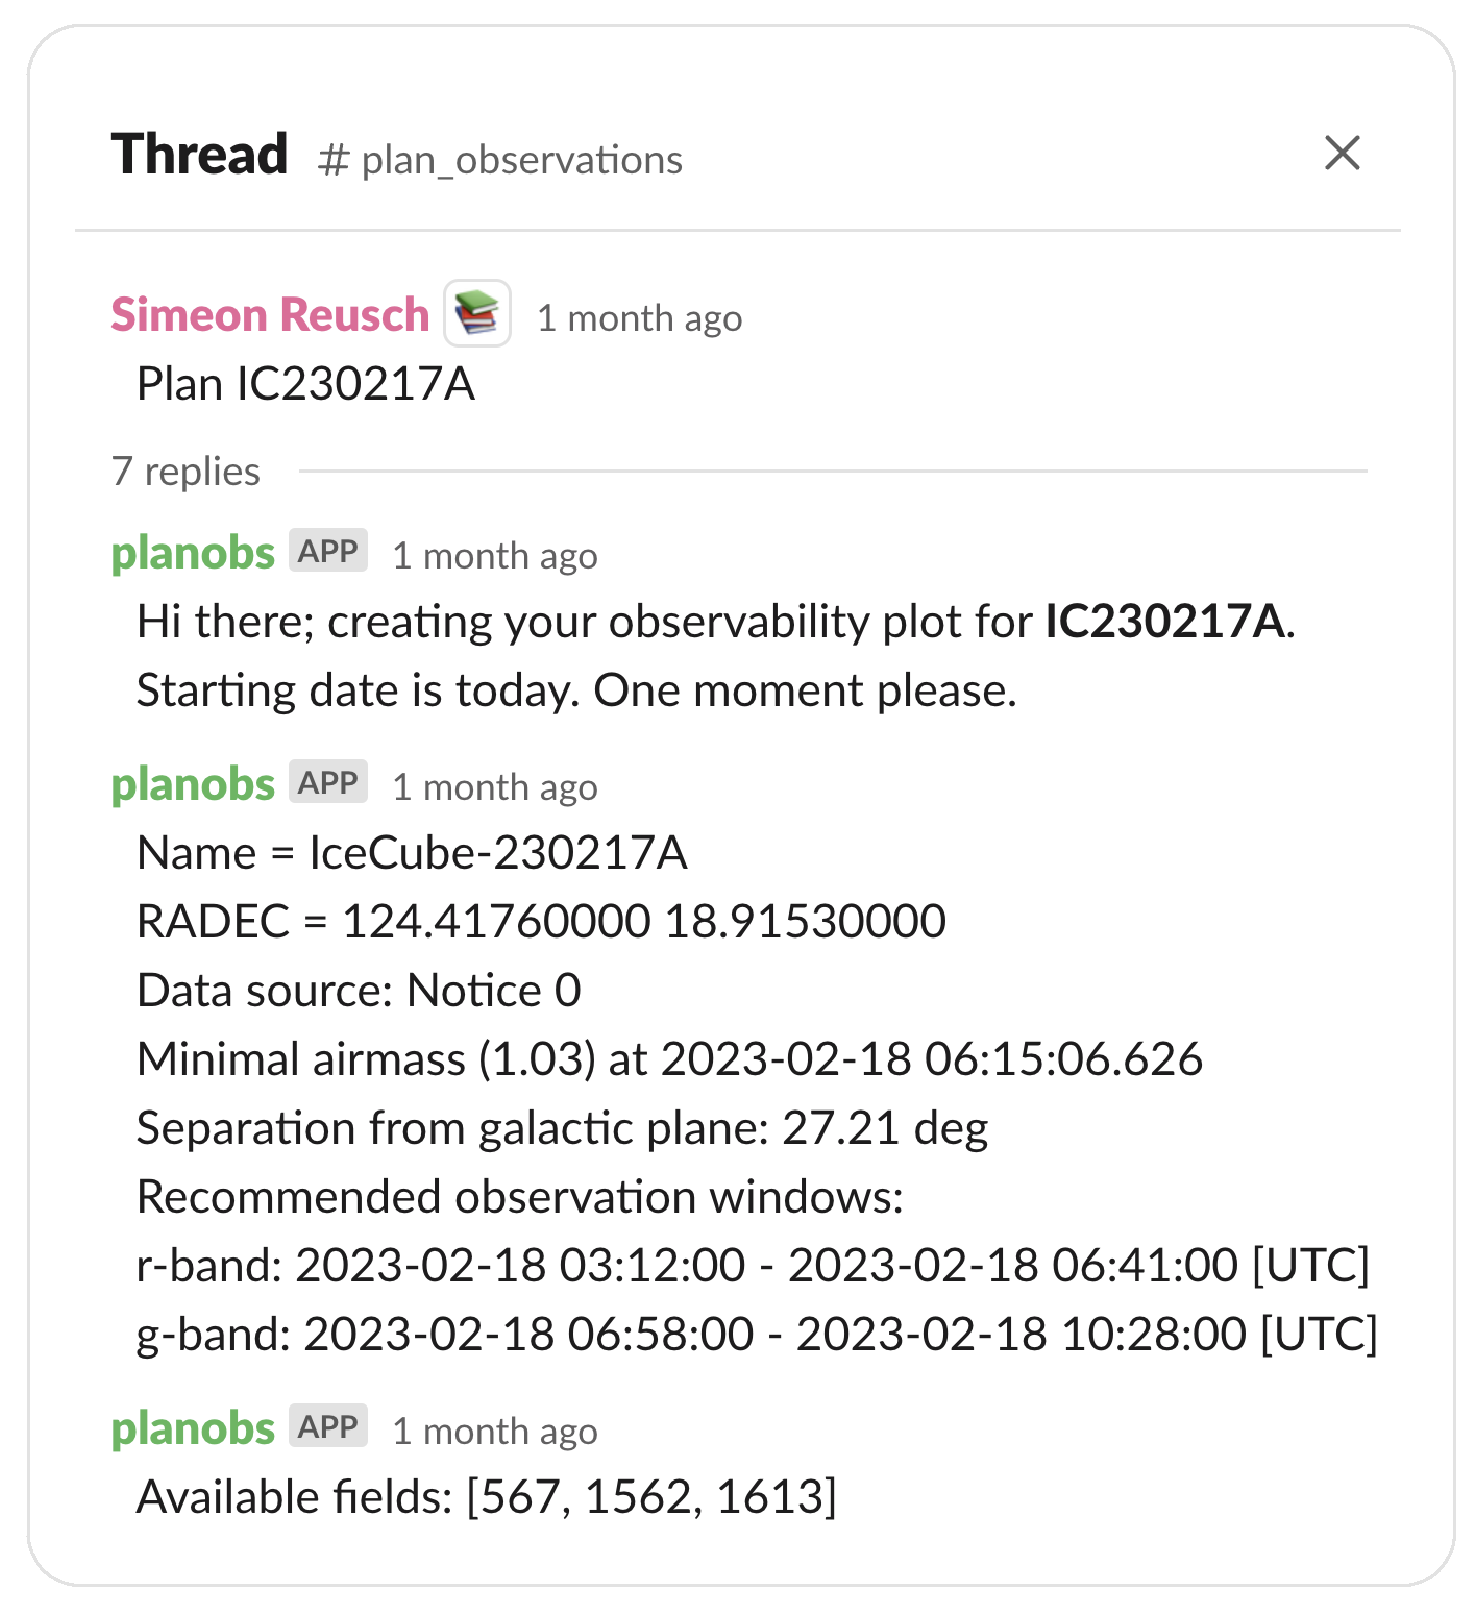
\includegraphics{fu/planobs_slack_border.pdf}
    \caption[\texttt{planobs} Slack interaction]{Sample interaction with \texttt{planobs} in Slack, checking the observability of IC230217A.}
    \labfig{planobs_slackbot}
\end{marginfigure}

If an alert makes these cuts, one needs to \textbf{check if observations with ZTF are feasible}, and create an observation plan. As we are interested in the \textbf{time evolution} of potential source candidates, usually observations within a 10 day window are triggered. To obtain deep images during the first night, we first trigger \SI{300}{\second} exposures in the \textit{g}- and \textit{r}-band. These are followed by shallower \SI{30}{\second} observations in the \textit{g}-band during nights 2, 3, 5 and 7, and finally shallow observations in both \textit{g}- and \textit{r}-band during night 9.



To reduce the potential for errors, the feasibility checks and creation of an observation schedule are done with the \texttt{planobs}~\sidecite{Reusch2023} tool, developed and maintained by the author to automate triggering follow-up observations as much as possible.

\texttt{planobs} is written in Python, and is deployed on a virtual private server. The backend runs on \texttt{Flask}\sidenote{\url{https://flask.palletsprojects.com}} behind a \texttt{nginx}\sidenote{\url{https://nginx.com}} reverse proxy exposed to the internet. The \texttt{nginx} endpoint serves a Slack\sidenote{\url{https://slack.com/}} bot integrated into the DESY multimessenger group chat for ease of use. It can also be run locally.

The tool is designed to be used with a simple command-line-style interface in the working-group Slack chat. For example, issuing
\begin{lstlisting}[language=bash,style=kaolstplain]
Plan IC221223A -multiday
\end{lstlisting}
in the \texttt{plan\_observations} Slack channel will create an observation plan for IceCube high-energy neutrino IC220501A.

To obtain the positional and error information on the neutrino in question from the respective GCN Circular, \texttt{planobs} is searching for the GCN on a server hosted by NASA\sidenote{\url{https://heasarc.gsfc.nasa.gov/wsgi-scripts/tach/gcn_v2/tach.wsgi}}. As circulars are written by humans, it fuzzily parses them to extract the relevant information. After this, observability at Mt. Palomar is calculated, defaulting to the current time (optionally, a desired observation time can be requested).

\begin{figure}[h!]
    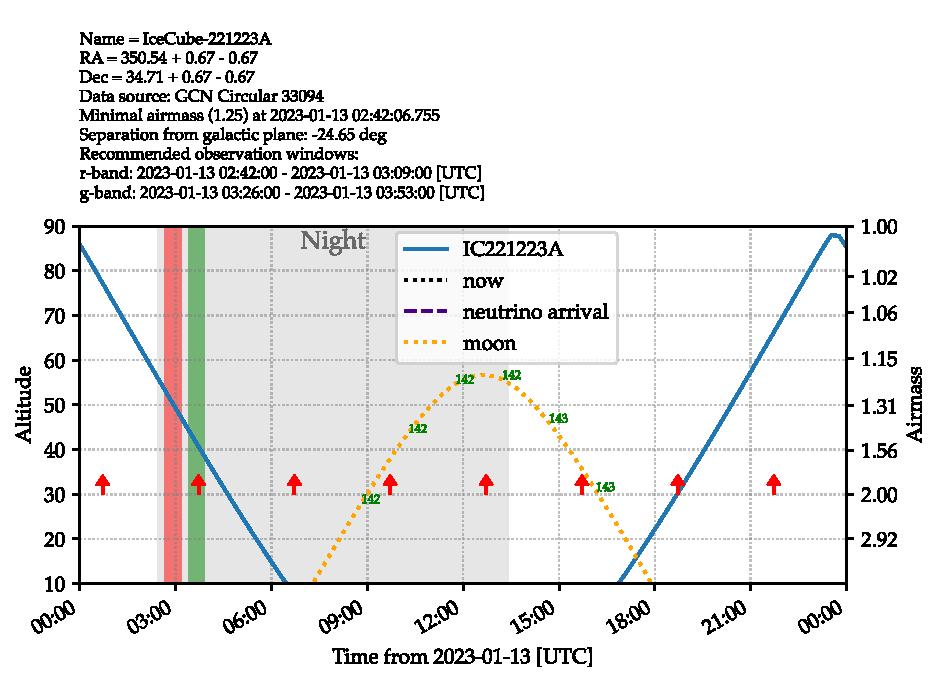
\includegraphics{fu/planobs_airmass.pdf}
    \caption[Observation plan]{Observation plot created by \texttt{planobs} for the follow-up of IceCube neutrino IC221223A. The altitude and airmass of the alert region at Mt. Palomar are shown in blue. The red and green shaded regions are proposed observation windows in the \textit{r}- and \textit{r}-band. The red arrows show the airmass limit of 2.0, and the moon is displayed as yellow dotted curve. The gray shaded region marks night-time at the telescope site. All information automatically extracted from the GCN Circular are shown on top.}
    \labfig{planobs}
\end{figure}

An example observability plot is shown in Fig.~\ref{fig:planobs}. The blue curve shows the altitude of the neutrino sky region above Mt. Palomar, and the red and green shaded regions mark the two proposed observation windows in the \textit{r}- and the \textit{g}-band.

\begin{marginfigure}
    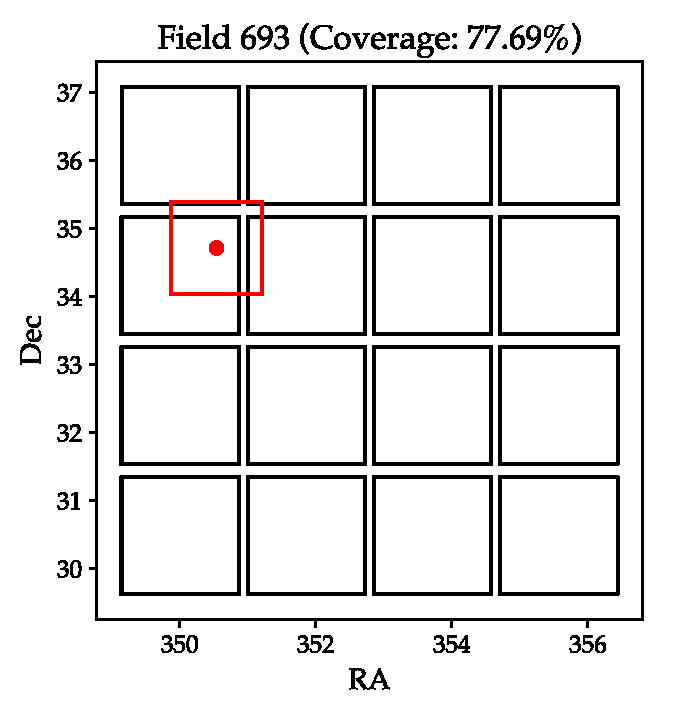
\includegraphics{fu/planobs_grid.pdf}
    \caption[\texttt{planobs} ZTF grid]{The bounding rectangle of the \SI{90}{\percent} uncertainty area of IC221223A overlayed onto the ZTF grid. The coverage does not equal \SI{100}{\percent} because chip gaps are taken into account.}
    \labfig{planobs_grid}
\end{marginfigure}

Additionally, for each field of the primary and secondary grid (see Section~\ref{ztf_grid}) that overlaps with the uncertainty region, \texttt{planobs} checks if reference images are available (see Section~\ref{ztf_image_subtraction}), calculates the resulting coverage and selects the field with the \textbf{highest coverage}. Fig.~\ref{fig:planobs_grid} shows such an overlay plot for IC221223A and ZTF field 693.

If the plan looks good, i.e.\ if the object is observable above an airmass of 2.0 and the moon is not too close, one needs to invoke

\begin{lstlisting}[language=bash,style=kaolstplain]
Plan IC221223A -trigger
\end{lstlisting}

to submit the observation request via a dedicated API to the ZTF telescope scheduler. There is additional functionality to ensure that the trigger has been added to the telescope queue. If all goes well and weather permits, the observations are carried out, and one can proceed to do candidate vetting.

\section{The \texttt{AMPEL} Broker}\label{ampel}

The next step in the pipeline is the \textbf{selection of good candidates}. ZTF typically serves 200000 alerts per night. As only a fraction of those is relevant for the neutrino follow up, we need software to cut down the number of alerts. This is exactly what \texttt{AMPEL}~sidecite{Nordin2019} is doing, a streaming data analysis framework developed at Humboldt-University Berlin and DESY Zeuthen with contribution of the author.

The main design goals of \texttt{AMPEL} comprise scalability, modularity and provenance tracking. It was built with the data rate of future Rubin observatory~\sidecite{Ivezic2019} in mind, and was subsequently selected as one of 7 brokers\sidenote{See \url{https://www.lsst.org/scientists/alert-brokers}.} for Rubin observatory. The full software stack is written in Python.

\begin{figure}[h!]
    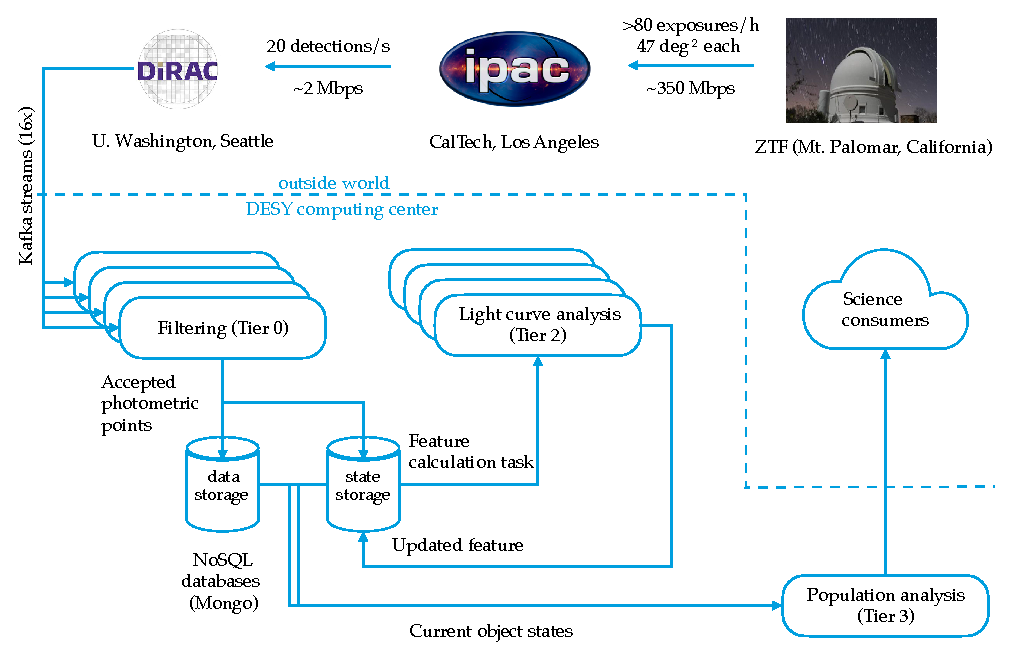
\includegraphics{fu/ampel_design.pdf}
    \caption[\texttt{AMPEL} overview]{Overview of the \texttt{AMPEL} data processing. Alerts from DiRAC are ingested into \texttt{AMPEL}, where they are processed, combined, analyzed and served to science consumers. From~\cite{Nordin2019}}
    \labfig{ampel_design}
\end{figure}

Fig.~\ref{fig:ampel_design} shows the design and information flow of \texttt{AMPEL}. On the top, data from Mt. Palomar is transmitted to IPAC (see Section~\ref{ztf_data_link}), where detections are extracted from the difference images. These are then sent to the Institute for Data Intensive Research in Astrophysics \& Cosmology (DiRAC) at the University of Washington, where they are distributed via parallel \texttt{Kafka} streams. This is the live data stream the ZTF instance of \texttt{AMPEL} listens to.

The first of several execution layers (\textit{tiers}) is the \textbf{Filtering} stage (Tier 0). Here, different filters can be implemented, reducing the large number of alerts by different criteria. These comprise e.g.\ \texttt{RealBogus} and \texttt{sgscore}\sidenote{See Section~\ref{ztf_image_subtraction}}, color evolution, host galaxy properties and the (non-) existence of a detection history. All alerts surviving the filtering stage are then stored in a \texttt{MongoDB}\sidenote{\url{https://mongodb.com}} database collection. Additionally, processing states are stored in another collection.

A description of \textbf{Tier 1} can be skipped here, as it serves mainly technical purposes (for details, see~\cite{Nordin2019}). The next relevant stage is the \textbf{Light curve analysis} stage (Tier 2). Here, additional information on the transients are either obtained or generated. Possible steps are querying external catalogs for host galaxy or redshift information, fitting lightcurves with various models or photometrically classify transients with machine learning~\cite{Nordin2019}.

The last level, tier 3, executes \textbf{Population analyses}. These are schedulable actions, triggered on request or at pre-defined times (ranging from yearly data dumps, through daily updates to nearly real-time execution). A typical use case is the automated ranking of different transients for a specific science goal. An example is the daily posting of new supernova candidates to a Slack channel, ranked by how promising they are for spectroscopic follow up~\cite{Nordin2019}.

To simplify matters significantly and to allow reprocessing as well as full replayability, all ZTF alerts received via the \texttt{Kafka} streams since June 2018 are also stored in an archival alert database hosted at DESY. The database is based on \texttt{Postgresql}\sidenote{\url{https://postgresql.org/}} and can be accessed via a web frontend and an API\sidenote{\url{https://ampel.zeuthen.desy.de/api/ztf/archive/v3/docs}}.

\section{Candidate Filtering with \texttt{nuztf}}
To streamline the neutrino follow-up process, \texttt{nuztf}~\sidecite{Stein2023} was created for filtering and inspecting candidate counterparts, with significant contribution by the author. It is written in Python, and relies heavily on \texttt{AMPEL} (see Section~\ref{ampel}). The main use case is the follow up of high energy neutrinos, but it can also handle skymaps from LIGO-Virgo-Kagra (LVK) gravitational wave (GW) alerts or GRB skymaps, and was used in the ZTF follow up campaign during the third observational campaign (O3) of Ligo and Virgo~\cite{Kasliwal2020}.

When run, \texttt{nuztf} executes the following steps: (1) It obtains the IceCube alert information from the GCN, (2) it constructs a \texttt{HEALPix} map from the \SI{90}{\percent} uncertainty rectangle, (3) it queries the \texttt{AMPEL} archive for all alerts within the \texttt{HEALPix} map\sidenote{Because the archive database contains \texttt{HEALPix} indices with different resolutions, this kind of query is much faster than a cone search.} in a given time range, (4) it applies the \texttt{AMPEL} \texttt{DecentFilter}~\cite{Nordin2019} with custom parameters (see below), (5) it crossmatches the surviving counterpart candidates to a list of catalogs, (6) it pushes the candidates to \texttt{Fritz}\sidenote{\url{https://fritz.science}} and (7) it creates an overview \texttt{pdf} file with details and a light curve for each candidate.

\subsection{\texttt{DecentFilter} Parameters}
The GCN parsing is done akin to \texttt{planobs} (see Section~\ref{planobs}). After extraction of the alert information and querying the Archive database with a \texttt{HEALPix} map, a first filter, \texttt{DecentFilter}, is run with the following parameters:
\begin{description}
    \item[Time window] The transient must have shown activity in a 14-day window after neutrino detection
    \item[\texttt{RealBogus}] The transient must have a \texttt{RealBogus} score of $>0.3$.
    \item[Positive subtraction] Sometimes, subtraction from reference images result in negative flux. This criterion ensures that there is excess flux.
    \item[Detections] The candidate must have at least 2 detections, separated by at least \SI{15}{\minute}. Note that this needs to be reflected in the observation planning.\ \texttt{planobs} (see Section~\ref{planobs}) takes care of that.
    \item[\texttt{sgscore}] The transient must have an \texttt{sgscore} $<0.8$, which means a low probability of being a star.
    \item[Maximum distance to PS1] As noted in Section~\ref{ztf_alerts}, the \texttt{sgscore} star-galaxy classifier is trained on data from PS1. To ensure correct association of the \texttt{sgscore} value which is based on the closest PS1 source, we require the source to be closer than \SI{1}{\degree}. The veto is also ignored if 3 PS1 sources are closer than \SI{3}{\degree} and their \texttt{sgscore} lies between $0.4$ and $0.6$, as this hints at possible PS1 source confusion.
    \item[Gaia star veto] Vetoes the source if the probability of it being a star is high, based on parameters from the Gaia survey.
\end{description}
The vast majority of alerts do not pass these filters, significantly reducing the human effort needed in candidate vetting.
\begin{marginfigure}
    \includegraphics{fu/nedz.pdf}
    \caption[NED spectroscopic redshift distribution]{Distribution of the 8.9 million NED objects with spectroscopic redshift (as of November 2021). From \url{https://ned.ipac.caltech.edu/Documents/Holdings/graphics}.}
    \labfig{nedz}
\end{marginfigure}
\subsection{Catalog Crossmatching}\label{catmatch}
All surviving candidates are then spatially crossmatched to a set of catalogs. These are:
\begin{description}
    \item[CRTS] A catalog derived from the Catalina Realtime-Transient Survey (CRTS)~\sidecite{Drake2009}, the Catalina Surveys Periodic Variable Star Catalog~\sidecite{Drake2014}, is queried to check if the source is a \textbf{variable star}.
    \item[Gaia] Gaia Data Release 2 (Gaia DR2)~\sidecite{Brown2018} is also used to crossmatch with known stars.
    \item[MILLIQUAS] The Million Quasar Catalog (MILLIQUAS)~\sidecite{Milliquas} contains 1.4 million quasi-stellar object (QSO) candidates. Crossmatching is done to see if the source candidate is most likely associated to an \textbf{AGN}.
    \item[NED] The NASA/IPAC Extragalactic Database (NED)\sidenote{\url{https://ned.ipac.caltech.edu}} hosts information on 1.7 billion objects, compiled from various surveys and catalogs. Almost 9 million of those have a \textbf{spectroscopic redshift}.
    \item[SDSS] Data Release 10 (DR10)~\sidecite{Ahn2014} of SDSS is used to check if the object is flagged as potential star.
    \item[TNS] The Transient Name Server (TNS)\sidenote{\url{https://wis-tns.org/}} is the repository of astrophysical transients and contains over 100k objects, both classified and unclassified. It is queried to check if the candidate source is a \textbf{known and possibly classified transient}.
    \item[WISE] Color information from the Wide-Infrared Survey Explorer (\textit{WISE}) Mission~\sidecite{Wright2010} can be used to identify likely AGN, as these predominantly occupy a small section of the WISE color-color diagram (see e.g.~\sidecite{Hviding2022} for this).
\end{description}
None of those catalog matches serve as veto, but are rather appended to the final output. This can be motivated by the insecure classification of Milliquas (QSOs) and SDSS (stars), which are partly derived from machine learning and therefore warrant human inspection. Also, some of the additional information can strengthen the case for a candidate source --- for example, an existing classification on TNS as a certain type of supernova.

\begin{figure}[h!]
    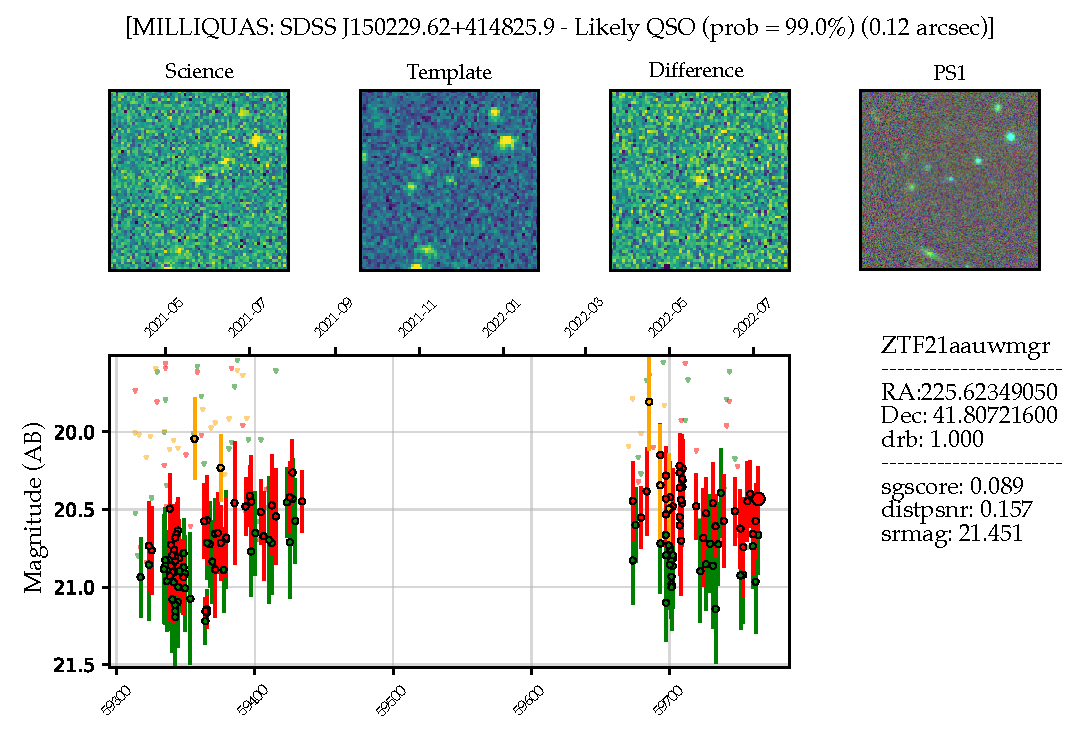
\includegraphics{fu/nuztf_IC220624A.pdf}
    \caption[\texttt{nuztf} output]{Sample output from \texttt{nuztf} showing the light curve of ZTF21aauwmgr, a transient selected as potential source in the follow up of IC220624A. The cutouts at the top show the science image, the reference image (template), the resulting difference image and a PS1 cutout of the same region. The bottom shows the transient light curve, as well as the position, the \texttt{RealBogus} score (\texttt{drb}) and the \texttt{sgscore}. On the top, crossmatching information is shown. Here, the source is a source discovered by SDSS and flagged as likely QSO in MILLIQUAS.}
    \labfig{nuztf_sample_output}
\end{figure}
Fig.~\ref{fig:nuztf_sample_output} shows a page from the final \texttt{pdf} file generated for neutrino IC220624A, displaying candidate source ZTF21aauwmgr. All information required for quickly deciding if the candidate warrants further scrutiny is displayed: \textbf{Image cutouts} of the science, reference and difference image are shown to allow identifying potential subtraction artifacts. The different \textbf{ML scores} (star-galaxy separation, real bogus) are also displayed, as well as results from the \textbf{catalog matching} and of course the transient \textbf{light curve}.

In addition the \texttt{pdf}, the draft of a GCN Circular is created, pre-filled with the observation times, the coverage and all final candidates to allow for quick distribution of promising sources. Also, all candidates passing the final round of filtering are pushed to the collaborative time-domain astronomy portal \texttt{Fritz} for bookkeeping and further discussion.

The code can either be run locally, or through the interaction with a Slackbot. This bot is hosted by the author on a virtual private server. The endpoint exposed to Slack is run with \texttt{gunicorn}\sidenote{\url{https://gunicorn.org}}, a Python WSGI server, behind an \texttt{nginx} reverse proxy. The bot can parse the names of Icecube alert neutrinos and gravitational wave event names, extract the information from the GCN or GW map and upload the overview \texttt{pdf} and the GCN draft to Slack.

\section{Forced Photometry with \texttt{fpbot}}\label{fpbot}
The last step in the pipeline is the acquisition of forced photometry. This is achieved with \texttt{fpbot}~\sidecite{Reusch2023a}, a forced photometry pipeline written by the author for ZTF, built upon on \texttt{ztflc}\sidenote{\url{https://github.com/mickaelrigault/ztflc}}.

\subsection{Forced Photometry Explained}
The usual extraction of transient flux, as performed by the ZTF imaging pipeline\sidenote{See Section~\ref{ztf_image_subtraction}}, cannot a priori know at which position to expect flux in the difference image. In the case of ZTF, there is a signal-to-noise threshold of $5$. If the flux detected at a position in the image exceeds that threshold, an alert is generated.

If the position of the transient is known, as it has already generated some alerts, one can \textbf{use this location to reprocess the difference images} and extract flux at precisely this position. With this method, one can extract a signal that is fainter than the signal-to-noise threshold. In most cases, this means that the transient can be detected at a younger age than its earliest alert photometry detection, or that the tail of the lightcurve of a fading transient can be detected longer. This process is dubbed \textbf{forced photometry}, as the known position is `forced' upon the flux extraction.

The possibility to extract flux prior to the first alert detection makes forced photometry especially useful to accept or reject some candidate neutrino sources: If e.g.\ a stripped-envelope supernova (that is compatible with high-energy neutrino production, see Section~\ref{ccsne}) shows an early forced photometry detection days prior to the neutrino arrival, the source can be rejected as candidate (see~.e.g\ Section~\ref{SN2020lls}).

\subsection{The \texttt{fpbot} Pipeline}
\begin{marginfigure}
    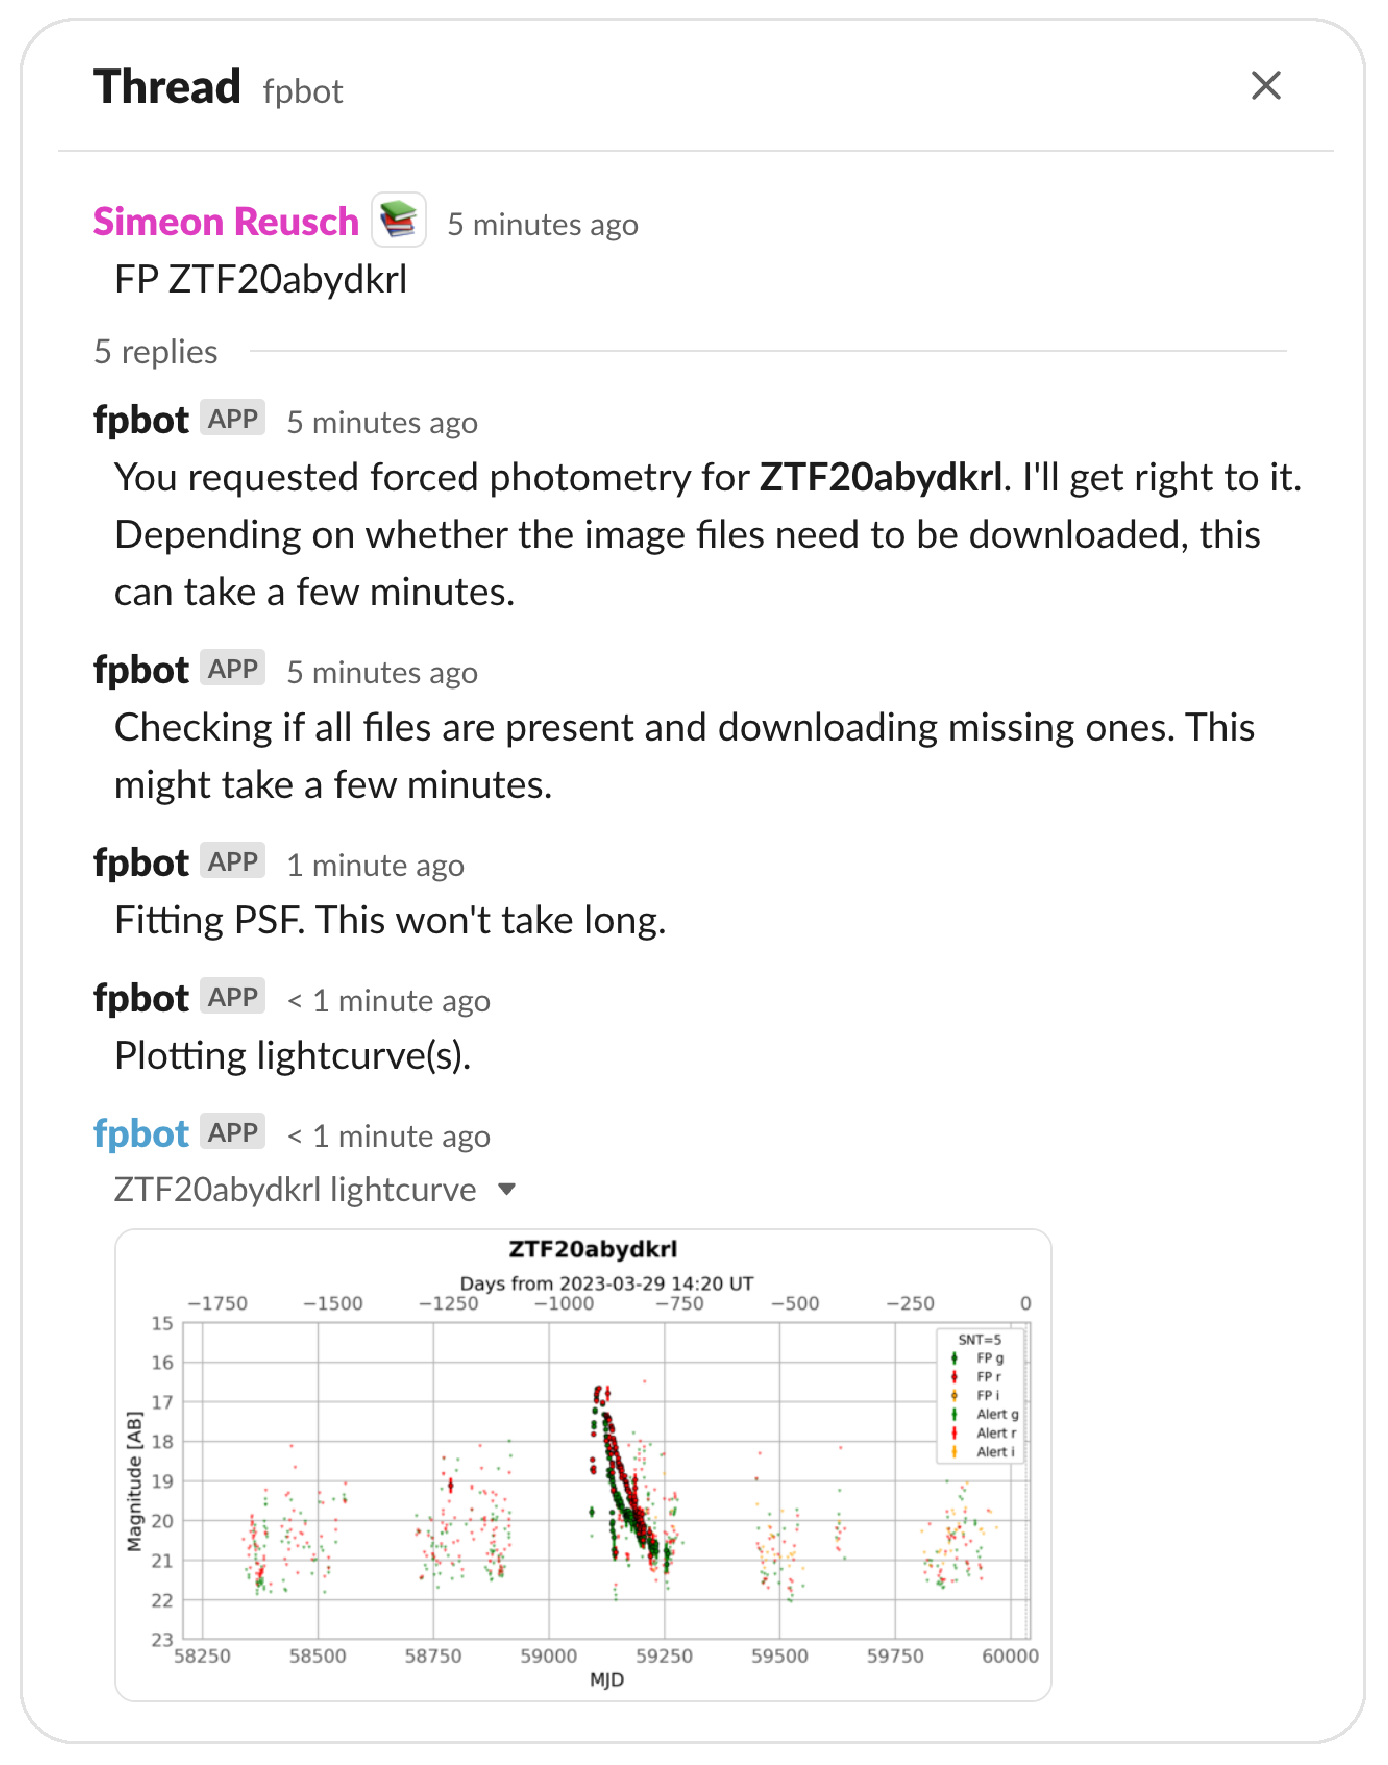
\includegraphics{fu/fpbot_slack_border.pdf}
    \caption[\texttt{fpbot} Slackbot interaction]{Sample interaction with the \texttt{fpbot} Slackbot, obtaining forced photometry for ZTF20abydkrl.}
    \labfig{fpbot_slackbot}
\end{marginfigure}
\texttt{fpbot} was written in Python by the author and provides a multi-threaded pipeline to obtain forced photometry extracted from ZTF difference images. It employs a \texttt{MongoDB} database to store the download and processing status for transients to avoid multiple downloads and unnecessary refits. Fitting requests can either be issued locally with a command-line interface, or within a dedicated Slack channel to serve the broader community.

For each object that is processed, first the \texttt{AMPEL} archive is queried for alerts of this object. From these, the median sky location is computed independently for each band (\textit{g}, \textit{r} and \textit{i}), as the stable astrometric solution deviated from band to band when testing the pipeline.

Difference image cutouts at the desired location as well as the PSF shape images are then downloaded from IPAC in parallel, maximizing throughput. After this stage, the \texttt{ztflc} package is used to measure the flux in the difference image cutout, given the median band location and the PSF image. This is done using the \texttt{iminuit} package~\sidecite{Dembinski2023}, running the least-square fit algorithm \texttt{MIGRAD}~\sidecite{James1975}.

The fit results are stored as \texttt{csv} files and returned either via Slack channel or email. If the forced photometry is requested of the same object again, only new epochs are fitted to speed up the process. The service is used also by the cosmology and supernova ZTF working groups.

\section{Spectroscopic Resources}\label{spec_resources}
To classify promising counterpart candidates, we have successfully submitted proposals for \textbf{spectroscopic resources} during the run of the neutrino follow-up program. Several of these were led by the author.

The instruments on which we had time for ToO observations during the last years comprise SEDM on the Palomar P60 telescope (\SI{1.5}{\meter}), the Alhambra Faint Object Spectrograph and Camera (ALFOSC) on the Nordic Optical Telescope (NOT, \SI{2.6}{\meter})~\sidecite{Djupvik2010}, the Device Optimized for the LOw RESolution (Dolores) on the Telescopio Nazionale Galileo (TNG, \SI{3.6}{\meter})~\sidecite{Mancini1997}, the Gemini Multi-Object Spectrograph (GMOS-N)~\sidecite{Hook2004} on the Gemini North Telescope (\SI{8.1}{\meter}), the Multi-Object Double Spectrograph (MODS)~\sidecite{Pogge2010} on the Large Binocular Telescope (LBT, 2x\SI{8.4}{\meter}), the Low-Resolution Imaging Spectrometer (LRIS)~\sidecite{Oke1995} on the W. M. Keck Observatory (Keck, \SI{10}{\meter}) and the Optical System for Imaging and low-Intermediate-Resolution Integrated Spectroscopy (OSIRIS)~\sidecite{Cepa2003} on the Gran Telescopio Canarias (GTC, \SI{10.4}{\meter}).

The image reduction pipelines used were either custom routines provided by the instrument, \texttt{pyraf}\sidenote{\url{https://github.com/iraf-community/pyraf}}, a Python wrapper to IRAF~\sidecite{Tody1986}, or \texttt{pypeit}~\sidecite{Prochaska2020}, a Python-based reduction package. The latter was used for NOT/ALFOSC, TNG/Dolores, Gemini/GMOS-N, LBT/MODS and GTC/OSIRIS, while \texttt{pyraf} was used for Keck/LRIS.

\section{Follow-Up Performance}
As of March 2023, we have followed up \textbf{34 of the 108 non-retracted high-energy neutrino alerts} issued by IceCube\sidenote{See Section~\ref{ic_alert_program}} since the start of the program, which amounts to \SI{31}{\percent} of all alerts. An overview is shown in Fig.~\ref{fig:follow_up_overview}. The majority of alerts not followed up were only visible during the day (\textit{Proximity to the sun}), or did not meet our alert quality criteria\sidenote{See Section~\ref{alert_cuts}}. The rest were either located too close to the galactic plane ($|b|\leq\SI{10}{\degree}$) or the telescope was on hold due to weather or technical problems.

\begin{figure}[h!]
    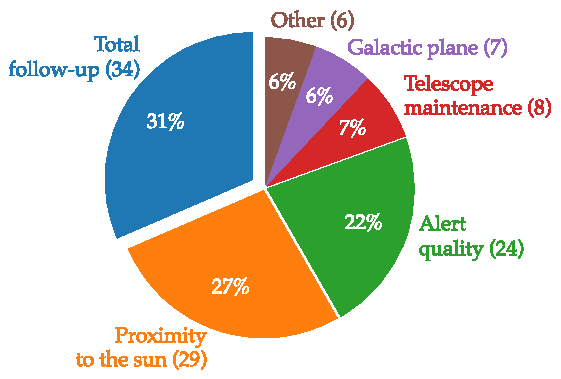
\includegraphics[width=0.7\textwidth]{fu/follow_up_overview.pdf}
    \caption[Follow-up performance]{Breakdown of the follow-up performance as of March 2023. Out of 108 neutrino alerts, 34 were followed up. The `Other' category comprises low altitude (below our airmass limit of 2.0 or entirely in the southern sky) and bad weather.}
    \labfig{follow_up_overview}
\end{figure}

An overview of all follow-up campaigns is shown in Table~\ref{tab:neutrino_alert_overview} in the appendix.
In total, 205 candidate sources were selected by \texttt{nuztf}. Of these, 27 (\SI{13}{\percent}) were distributed via GCN Circulars. The classification of these candidates will be discussed in Section~\ref{SN2020lls}.

Additionally, the follow-up performance over time is displayed in Fig.~\ref{fig:follow_up_summary}, with the followed-up alerts shown in green. As one can see, the performance has slightly deteriorated in the last two years, which can be mostly attributed to telescope downtime due to maintenance or technical faults.

\begin{figure}[h!]
    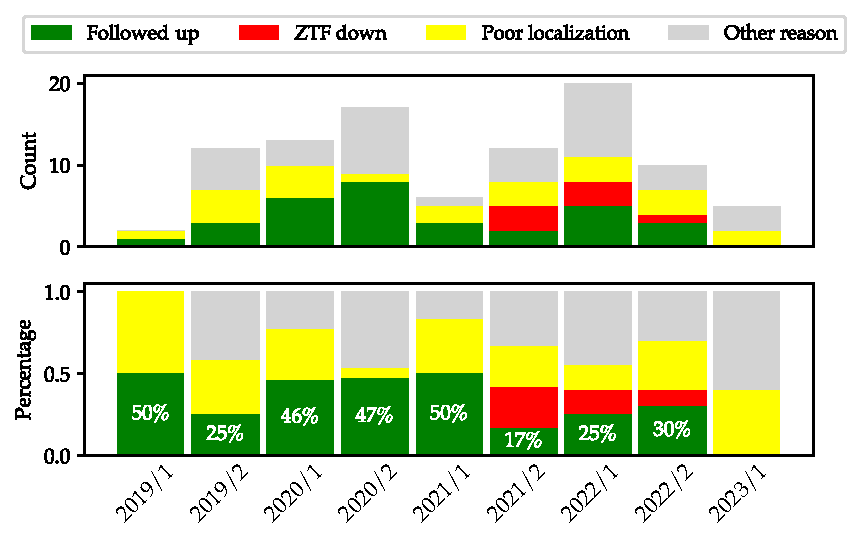
\includegraphics[width=1\textwidth]{fu/follow_up_summary.pdf}
    \caption[Follow-up performance over time]{Follow-up performance over time. The alerts we did follow-up on are shown in green, while poorly localized alerts not meetin our quality cuts are shown in yellow, and all other rejection reasons are shown in gray.}
    \labfig{follow_up_summary}
\end{figure}

\section{Notable Sources}
A full overview over the first 24 follow-up campaigns can be found in~\sidecite{Stein2023a}. In the following, those sources will be highlighted to which the author contributed either by requesting spectroscopic observations, reducing spectra or vetting candidates.

\subsection{\emph{SN2020lls}: Type Ic Supernova}\label{SN2020lls}
SN2020lls was identified in coincidence with high-energy neutrino \emph{IC200530A}~\sidecite{IC200530A1}. \SI{87}{\percent} (\SI{22.05}{\square\deg}) of the \SI{90}{\percent} rectangular uncertainty area were serendipitiously observed by ZTF roughly \SI{10}{\minute} after the neutrino detection. These observations were later appended by deep \SI{300}{\second} observations Three candidate sources were identified, including \emph{SN2020lls}~\sidecite{IC200530A2, IC200530A4}.

We took a spectrum of \emph{SN2020lls} with NOT/ALFOSC on June 12, 2020 and used the Supernova Identification (\texttt{SNID}) code~\sidecite{Blondin2007} to fit spectra of different types supernovae to the spectrum. The best fit spectrum was a \textbf{Type Ic supernova} at redshift $z=0.041$, 14 days post peak. The spectrum and the template are shown in Fig.~\ref{fig:ZTF20abdnpdo_spectrum}.

\begin{figure}[h!]
    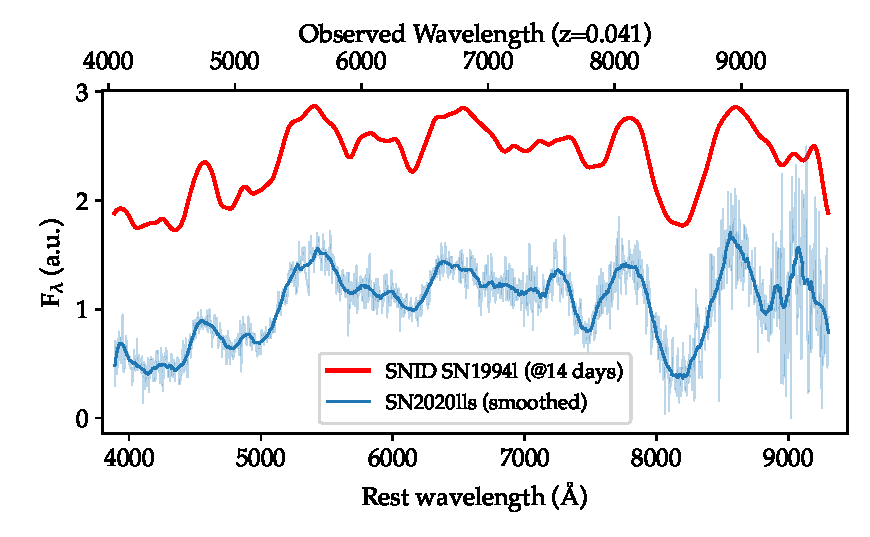
\includegraphics[width=1\textwidth]{fu/ZTF20abdnpdo_not_spectrum.pdf}
    \caption[SN2020lls spectrum]{Spectrum of SN2020lls taken with NOT/ALFOSC. The smoothed spectrum is shown in blue on the bottom, while the template spectrum of the Ic type supernova \emph{SN1994l} is shown on top in red. Figure by the author, see also~\cite{Stein2023a}.}
    \labfig{ZTF20abdnpdo_spectrum}
\end{figure}
SNe Ic are possible emitters of neutrino, but only shortly after explosion time (see Section~\ref{ccsne}). We therefore used the Modular Open Source Fitter for Transients (\texttt{MOSFiT})~\sidecite{Guillochon2018} to fit the light curve. The light curve, including an early forced photometry detection in the \textit{i}-band, can be seen in Fig.~\ref{fig:ZTF20abdnpdo_mosfit}.

\begin{figure}[htb]
    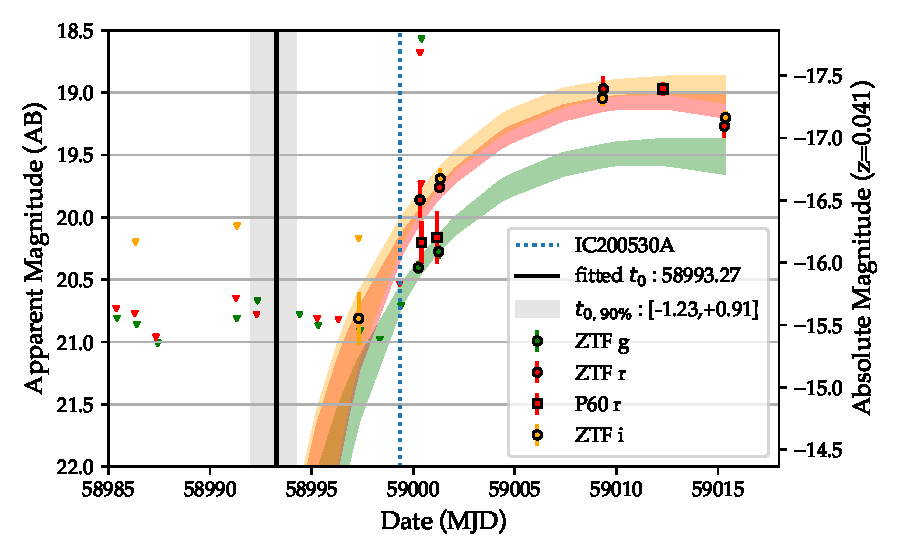
\includegraphics[width=1\textwidth]{fu/ZTF20abdnpdo_mosfit.pdf}
    \caption[\emph{SN2020lls} light curve fit]{Light curve of \emph{SN2020lls}. Detections are are filled circles or squares, while upper limits are shown as triangles. The early forced photometry detection in the \textit{i}-band constrains the explosion time estimated by \texttt{MOSFiT} fairly well to a time days prior (black line) to the detection of the neutrino (blue dotted line). This rules out \emph{SN2020lls} as candidate source. Figure by the author, from~\cite{Stein2023a}.}
    \labfig{ZTF20abdnpdo_mosfit}
\end{figure}
As can be seen, the fit estimates the explosion time (black line) at \textbf{6 days earlier} then the neutrino arrival time (blue dotted line). This allowed us to rule out \emph{SN2020lls} as source of \emph{IC200530A}.

\subsection{\emph{SN2020lam}: Type IIP SN without CSM-interaction}\label{SN2020lam}
A second source candidate that was also coincident with \emph{IC200530A}, was \emph{SN2020lam}~\sidecite{IC200530A3} with a supernova-like light curve. To obtain a classification, we took a spectrum with NOT/ALFOSC on June 6, 2020. Template fitting with \texttt{SNID} and \texttt{GELATO}~\sidecite{Harutyunyan2008} identified the source as a supernova of type IIP (see Fig.~\ref{fig:ZTF20abbpkpa_not_spectrum}).

\begin{figure}[h!]
    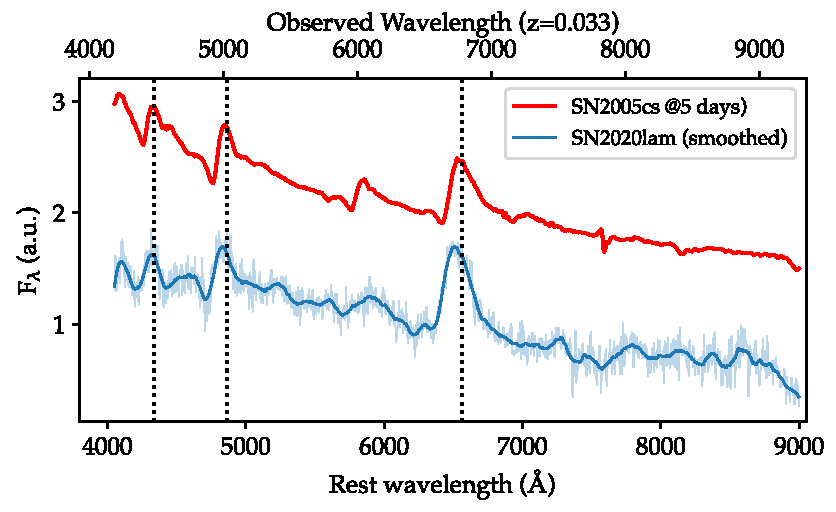
\includegraphics[width=1\textwidth]{fu/ZTF20abbpkpa_not_spectrum.pdf}
    \caption[\emph{SN2020lam} spectrum]{Spectrum of \emph{SN2020lam} taken with NOT/ALFOSC. The smoothed spectrum is shown in blue on the bottom, while the template spectrum of the IIP type supernova \emph{SN2005cs} is shown on top in red. Balmer lines are shown with black dotted lines. Figure by the author, see also~\cite{Stein2023a}.}
    \labfig{ZTF20abbpkpa_not_spectrum}
\end{figure}

The lightcurve and the best-fit template show that the neutrino was detected close to the peak of the supernova, a \textbf{Type IIP}. The viable production mechanism in this case is CSM-interaction (see Section~\ref{interacting_sne}). As the spectrum showed \textbf{no narrow lines}, we inferred that there is no sign of CSM interaction, and thereby ruled out \emph{SN2020lam} as a source candidate.

\subsection{\emph{AT2020ybb}: Unclassified}
\emph{AT2020ybb} was discovered when following up \emph{IC201021A}~\sidecite{IC201021A1}. Observations of the sky area started \SI{44}{\hour} after the neutrino detection and covered \SI{91}{\percent} (\SI{6.3}{\square\deg}).

\emph{AT2020ybb} was a promising candidate, as the light curve of the source was compatible with a supernova around peak~\sidecite{IC201021A2}. The other possibility was AGN activity, as the source was flagged as QSO with \SI{98}{\percent} probability within Milliquas.

We triggered GTC/OSIRIS and reduced the spectrum with \texttt{pyraf}. The spectrum is shown in Fig.~\ref{fig:ZTF20acmxnpa_spectrum}. Unfortunately, the spectrum did not allow a robust classification of the source, \textbf{neither confirming nor rejecting the neutrino source hypothesis}. If the line observed at \SI{7293}{\angstrom} is interpreted as SII, the resulting redshift is $z=0.087$.

\begin{figure}[htb]
    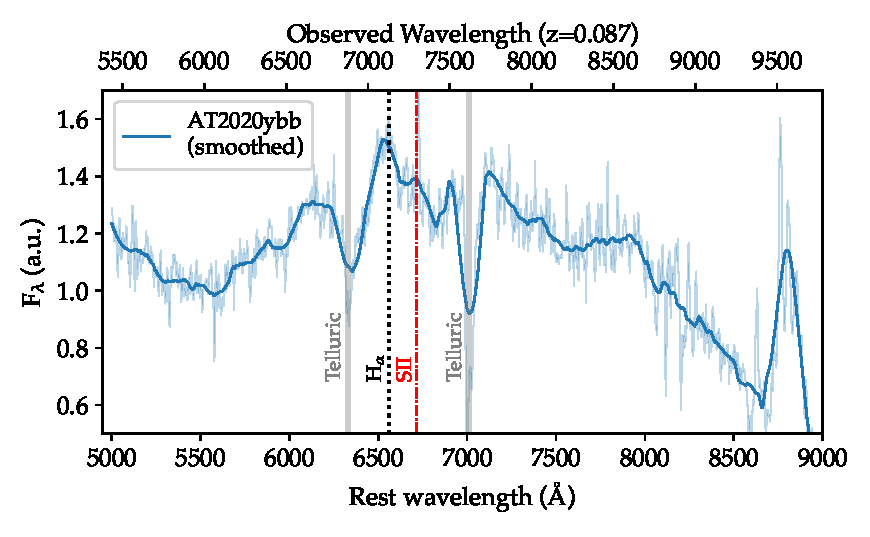
\includegraphics[width=1\textwidth]{fu/ZTF20acmxnpa_spectrum.pdf}
    \caption[\emph{AT2020ybb} spectrum]{Spectrum of \emph{AT2020ybb} taken with GTC/OSIRIS. The telluric absorption regions are shown in gray, potential hydrogen and SII lines are shown in black and red. The resulting redshift is $z=0.087$; the spectrum allowed no source classification.}
    \labfig{ZTF20acmxnpa_spectrum}
\end{figure}

\subsection{\emph{AT2021osi}: Regular AGN Activity}
\emph{AT2021osi} was detected when following up \emph{IC210629A}~\sidecite{IC210629A1}. It was first reported by \texttt{ALeRCe}~\sidecite{SanchezSaez2021}, about two weeks prior to the neutrino's arrival.

The proximity of the source to the nucleus of its host galaxy stipulated a TDE origin~\sidecite{IC210629A2}. To classify the transient, we triggered two \SI{750}{\second} observations with Gemini/GMOS-N and reduced the spectrum with \texttt{pypeit}.

The spectrum showed features typical for AGN, most importantly broad Balmer lines ($\text{H}_\alpha$, $\text{H}_\beta$ and $\text{H}_\gamma$). These allowed also to infer a redshift of $z=0.194$~\sidecite{IC210629A3}. As there was no contemporaneous flaring activity in the optical light curve, we ruled out this candidate as \textbf{regular AGN activity}\todo{need small section on FU classes at the beginning}.

\begin{figure}[htb]
    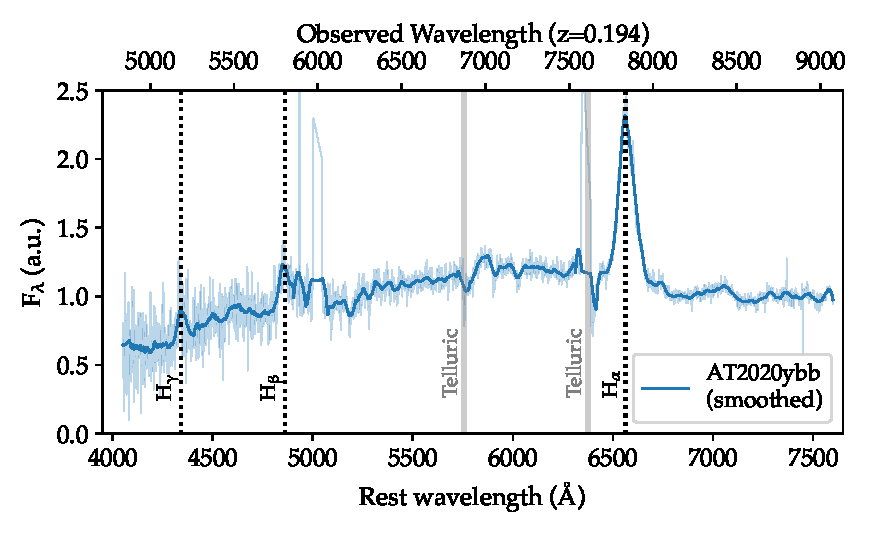
\includegraphics[width=1\textwidth]{fu/ZTF21abecljv_spectrum.pdf}
    \caption[\emph{AT2020osi} spectrum]{Spectrum of \emph{AT2020osi}, taken with Keck/GMOS-N. The telluric absorption areas are shown in gray, and Balmer lines are shown as black dotted lines. The redshift is $z= 0.194$, and we classified the source as AGN.}
    \labfig{ZTF21abecljv_spectrum}
\end{figure}


\subsection{SN2022oyn: Type Ia Supernova}
When following up \emph{IC220907A}~\sidecite{IC220907A1}, \emph{SN2022oyn} emerged as notable source candidate, as its light curve was consistent with a supernova about 40 days post peak~\sidecite{IC220907A2}.

We obtained a spectrum with Keck/LRIS on September 20, 2022. Based on a fit with \texttt{SNID} (see Fig.~\ref{fig:ZTF22aatwsqt_spectrum}), we classified the source as \textbf{Type Ia supernova}. It can therefore be ruled out as neutrino source, as SNe Ia are not predicted to emit high-energy neutrinos (see Section~\ref{sne_ia}).

\begin{figure}[htb]
    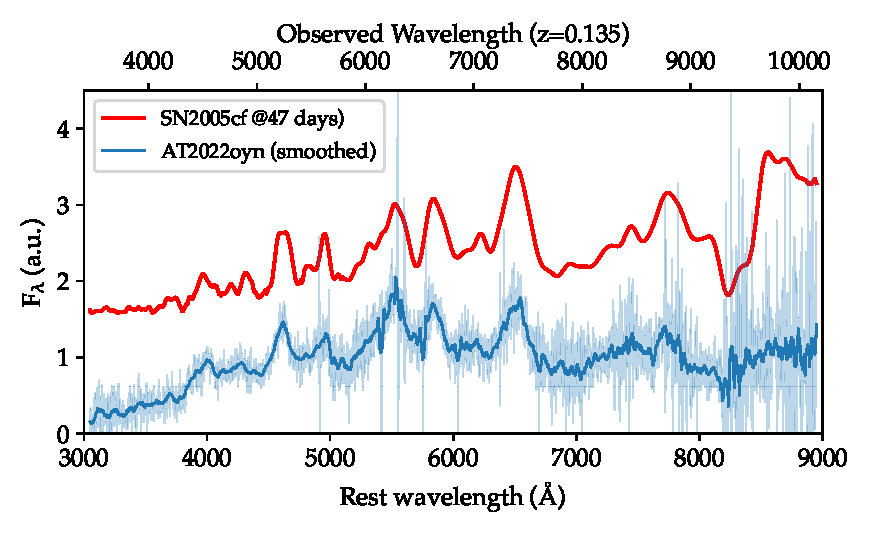
\includegraphics[width=1\textwidth]{fu/ZTF22aatwsqt_spectrum.pdf}
    \caption[\emph{SN2022oyn} spectrum]{Spectrum of \emph{SN2022oyn}, taken with Keck/LRIS. The best-fit \texttt{SNID}template (\emph{SN2005cf}), a SN Ia, is shown for comparison in red on top. The redshift inferred from the tempmlate match is $z=0.135$.}
    \labfig{ZTF22aatwsqt_spectrum}
\end{figure}

\subsection{TDE \emph{AT2019dsg}}\label{at2019dsg}
The author did not contribute to the analysis of the TDE \emph{AT2019dsg}, but as it is important in the context of the work on \emph{AT2019fdr} highlighted in the next Chapter (\ref{at2019fdr}), the most important findings will be presented in this section.

\emph{AT2019dsg} was identified as a possible counterpart to \emph{IC191001A}, an alert with a \SI{90}{\percent} bounding rectangle of \SI{25.5}{\square\deg}, an estimated neutrino energy of \SI{217}{\tera\eV} and a signalness\sidenote{See Section~\ref{ic_event_selection}} of 0.59~\sidecite{IC191001A1, IC191001A2}.

\emph{AT2019dsg} was already classified as TDE and was 6 months old at the time of neutrino arrival, peaking in the ZTF \textit{g}-band on May 3, 2019 (151 days prior to the neutrino). As a ZTF-detected TDE, it had already been observed by the Ultra-Violet/Optical Telescope (UVOT)~\sidecite{Roming2005} aboard NASA's \textit{Neil Gehrel's Swift Observatory} (\textit{Swift})~\sidecite{Gehrels2004}. These observations revealed bright UV emission, tracing the optical light curve of \emph{AT2019dsg} (see Fig.~\ref{fig:at2019dsg_lc}).

The blackbody temperature that can be inferred from the optical/UV was measured at \SI[parse-numbers = false]{10^{4.6}}{\K}, which is a bit higher than typical for TDEs~\sidecite{Stein2021}. Together with the transient redshift of $z=0.0512$, a peak luminosity of \SI[parse-numbers = false]{10^{44.5}}{\erg\per\s} can be calculated, which renders \emph{AT2019dsg} \textbf{one of the most luminous TDEs} discovered so far.


\begin{figure*}[htb]
    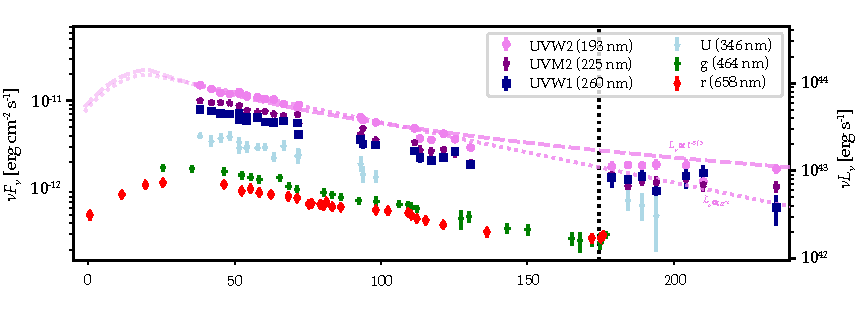
\includegraphics{fu/at0219dsg_lc.pdf}
    \caption[AT2019dsg optical/UV light curve]{Optical and UV light curve of AT2019dsg. The neutrino arrival time of IC191001A is marked with a black dotted line. From~\cite{Stein2021}}
    \labfig{at2019dsg_lc}
\end{figure*}

Furthermore, \emph{AT2019dsg} was observed by the X-ray Telescope (XRT)~\sidecite{Burrows2005} aboard Swift, starting about 40 days after discovery. Observations reveiled a \textbf{bright source that quickly faded to non-detection} within the next 30 days~\cite{Stein2021}. Possible explanations for this are either cooling of the newly formed accretion disk, or some kind of obscuration along the line of sight. The X-ray detection of AT2019dsg is not uncommon: 9 of the 30 TDEs detected during Phase I of ZTF operations have been detected in X-rays~\sidecite{Hammerstein2022}.

More peculiar, \emph{AT2019dsg} has also been detected in \textbf{radio wavelengths}. Observations by the Large Array of the Arcminute MicroKelvin Imager (AMI)~\sidecite{Zwart2008,Hickish2018}, MeerKAT~\sidecite{Jonas2018} and the Karl G. Jansky Very Large Array (VLA)~\sidecite{Thompson1980} at several different epochs following the neutrino detection showed a radio signal with temporal evolution over the course of the next months.

In~\cite{Stein2021}, the evolving radio signal was interpreted as the signature of a mildly relativistic outflow launched by the TDE. This interpretation was later disputed:~\sidecite{Cendes2021} added later radio observations to the dataset and found the radio data more compatible with a non-relativistic outflow, excluding neutrino production.~\sidecite{Mohan2022} performed very-long-baseline interferometry (VLBI) and also concluded on a non-relativistic outflow as the origin of the radio emission, while emphasizing the compatibility of that scenario with high-energy neutrino production. Nonetheless, the observations confirm \textbf{long-lived non-thermal emission} from the transient.

\begin{figure}[htb]
    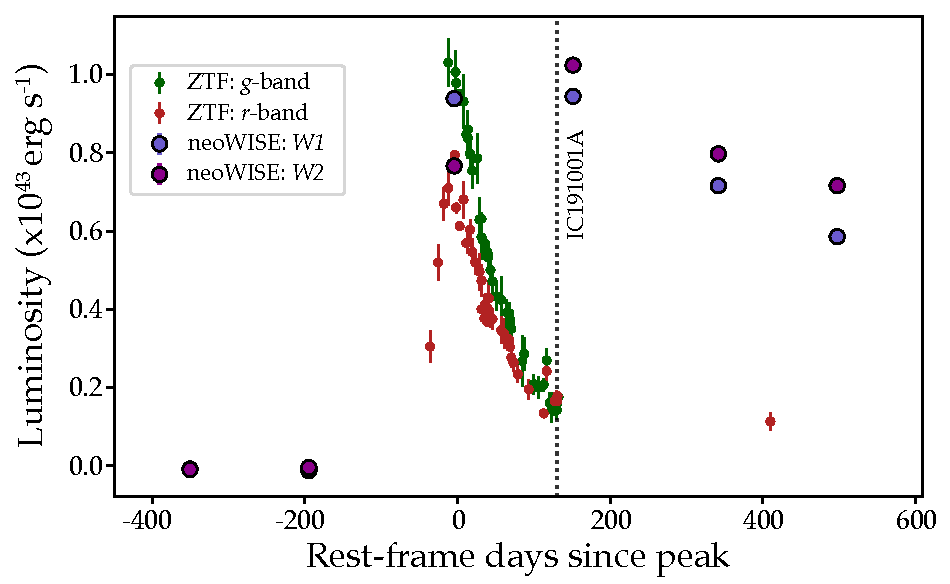
\includegraphics[width=1\textwidth]{fu/at2019dsg_dustecho.pdf}
    \caption[AT2019dsg infrared light curve]{AT2019dsg light curve with the \textit{WISE} infrared datapoints shown as bigger violet and magenta circles. From~\cite{Reusch2023b}.}
    \labfig{at2019dsg_dustecho}
\end{figure}

Lastly, a \textbf{strong infrared signal} was detected when evaluating \text{NEOWISE}~\sidecite{Mainzer2011} data that was not yet published at the time the source paper was finalized. The two \textit{WISE} bands can be seen in Fig.~\ref{fig:at2019dsg_dustecho}. The infrared flare trails the optical evolution --- this can interpreted as a \textbf{dust echo}, where the optical to X-ray light is reprocessed by surrounding dust, re-emitting it at infrared wavelengths after a delay introduced by the light travel time. This will be discussed in detail in Section~\ref{dust_echo} in the context of \emph{AT2019fdr}, the second neutrino associated TDE.

The \textbf{chance coincidence} to observe a high-energy neutrino in spatial and temporal coincidence with a radio-emitting TDE like \emph{AT2019dsg} was computed to be \SI{0.5}{\percent}, while the probability of finding one with a bolometric flux as high as \emph{AT2019dsg} was \SI{0.2}{\percent}~\cite{Stein2021}. This suggests that \textbf{Tidal Disruption Events do in fact contribute to the flux of high-energies measured by IceCube}.

Lightning rarely strikes twice. So the case that we identified \emph{AT2019fdr} as the second likely neutrino-associated TDE candidate half a year later further strenghtened the case for a TDE-neutrino connection. The next Chapter~\ref{at2019fdr} is dedicated to that event.

\section{Classification Performance}\label{classification_performance}

\begin{figure*}[htb]
    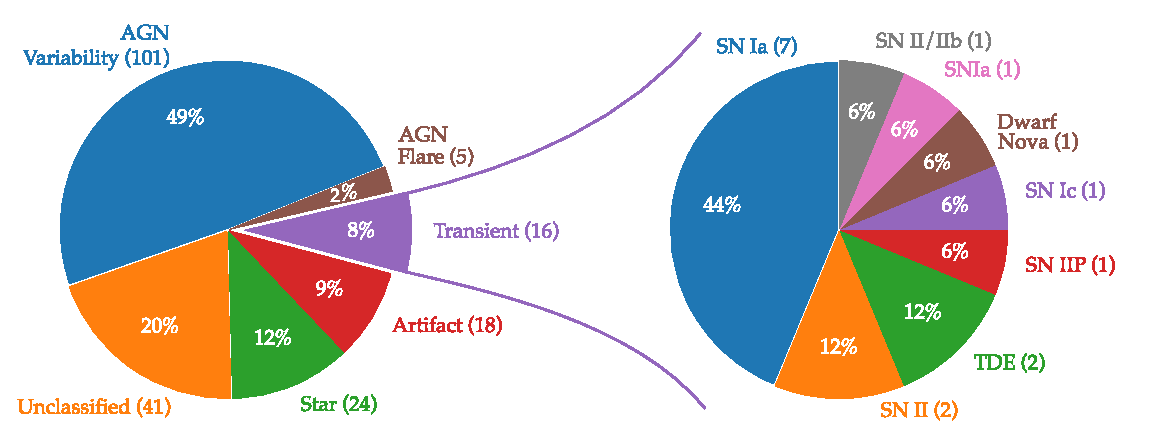
\includegraphics{fu/classification.pdf}
    \caption[Follow-up classification overview]{Overview of the classification performance of the neutrino follow-up program as of March 2023. The figure on the left shows all transients, while the figure on the right only show the subclasses of the \textit{Transient} category.}
    \labfig{classification_overview}
\end{figure*}

The classification for the \textbf{205 candidates selected} by \texttt{nuztf} can be seen in Fig.~\ref{fig:classification_overview}. The vast majority of transients has some kind of classification. Some of these classifications stem from spectroscopic follow up performed by us. In some cases, promising candidates were already spectroscopically classified by the ZTF Bright Transient Survey (BTS)~\sidecite{Fremling2020,Perley2020}, which aims to classify every transient detected by ZTF brighter than 19 mag. The rest of the classifications stem from catalog matches (.e.g\ Milliquas or Gaia, see Section~\ref{catmatch}).



Roughly half of the transients were classified as \textbf{AGN Variability}, i.e.\ stochastic AGN activity without a prominent optical flare visible around the time of neutrino detection. \SI{12}{\percent} (24) of the candidates were classified as \textbf{stars}, and hence ruled out as potential neutrino emitters. We classified \SI{9}{\percent} (18) of alerts as \textbf{subtraction artifacts}, as their difference images showed clear signs of erroneous subtractions\sidenote{See Section~\ref{ztf_image_subtraction}}. For \SI{20}{\percent} (41) of the candidates we were not able to obtain classifications.

This leaves 5 candidates that were classified as AGN, but did show coincident optical flares, as well as 16 bona fide \textbf{transients}, totalling 21 classified candidates.

Most of the classified candidates were SNe Ia. This is not surprising, as the majority of transients detected by ZTF are SNe Ia, due to their intrinsic brightness\sidenote{As of April 2023, \SI{63}{\percent} of all classified transients in BTS were SNe Ia.}. Among the other transients, only \textbf{the two TDEs were identified as source candidates}; these will be detailed subsequently. The remaining non-Ia supernovae could be \textbf{ruled out as potential sources}, as they either showed no sign of CSM interaction, or --- in the case of the SN Ic --- the explosion predated the neutrino detection significantly\sidenote{See Section~\ref{SN2020lls}}.

